\documentclass[tikz]{standalone}
\usepackage{tikz}
\usetikzlibrary{shapes}
\usetikzlibrary{positioning}
\usetikzlibrary{patterns}

\usepackage{newpxtext,newpxmath}
\usepackage{xcolor}

\definecolor{beaverorange}{HTML}{D73F09}
\definecolor{C0}{HTML}{1f77b4}
\definecolor{C1}{HTML}{ff7f0e}
\definecolor{C2}{HTML}{2ca02c}
\definecolor{C3}{HTML}{d62728}
\definecolor{C4}{HTML}{9467bd}
\definecolor{C5}{HTML}{8c564b}

\usepackage{siunitx}

\begin{document}



\begin{tikzpicture}

    \node[inner sep=0pt] (stargeom) at (0,0)
        {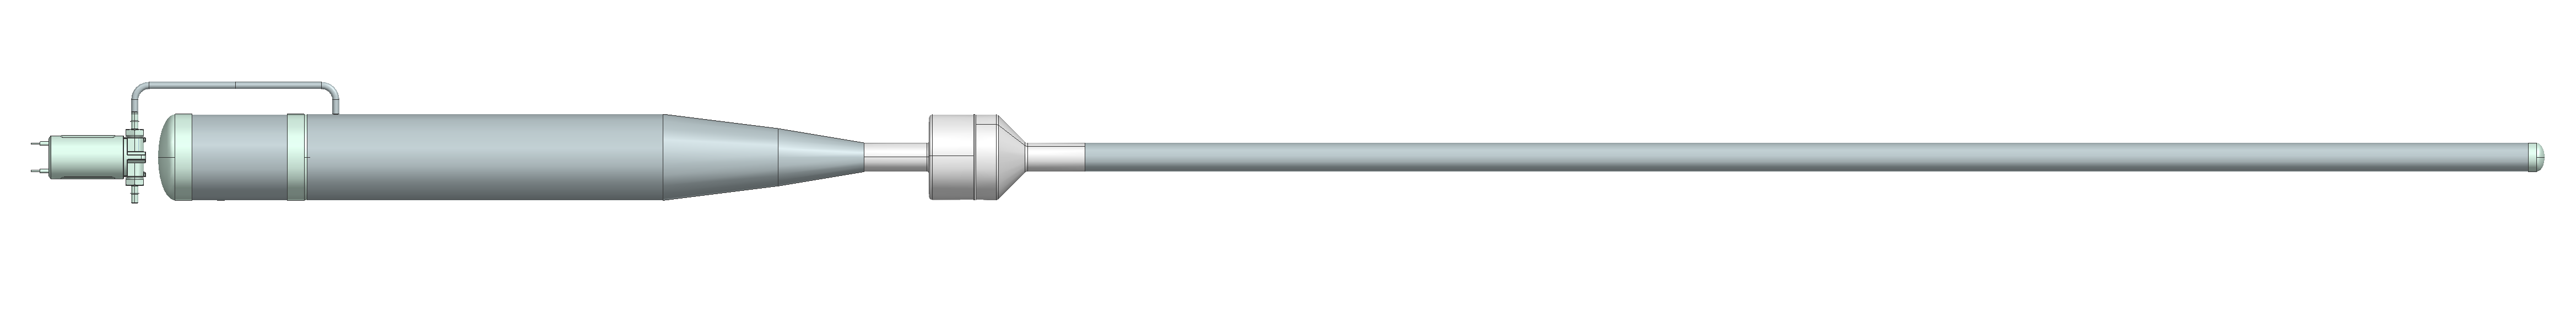
\includegraphics[width=15cm]{../figures/CAD-OSTR-Experiment.png}};
    
    \foreach \x in {7.3,-1.2,-2.5,-5.75,-6.55} {
        \draw[black,thin,dashed] (\x,-0.2) -- (\x,-0.75);
    }
    \draw[black,latex-latex] (7.3,-0.8) -- node[below]{\centering \SI{68.83}{\centi\meter}} (-1.2,-0.8);
    \draw[black,latex-latex] (-1.2,-0.8) -- node[below]{\centering \SI{10.4}{\centi\meter}} (-2.5,-0.8);
    \draw[black,latex-latex] (-2.5,-0.8) -- node[below]{\centering \SI{24.9}{\centi\meter}} (-5.75,-0.8);
    \draw[black,latex-latex] (-5.75,-0.8) -- node[below]{\centering \SI{3.41}{\centi\meter}} (-6.55,-0.8);





\end{tikzpicture}


\end{document}